\section{Theorie}
\label{sec:Theorie}

Zur Bestimmung der Elementarladung wird die Öltröpfchenmethode verwendet. 
In diesem Versuch werden Öltröpfchen zerstäubt und zwischen die Platten eines Plattenkondensators gesprüht.
Beim Einsprühen erfahren die Tröpfchen eine Reibung, die dazu führt, dass die Öltröpfchen elektrisch geladen werden.
Die Ladung einzelnen Tröpfchen entspricht einem ganzzahligen Vielfachen der Elementarladung $e$.
Befinden sich die Öltröpfchen zwischen den Kondensatorplatten, wirken ein oder mehrere Kräfte auf diese. 
Die konstante Gravitationskraft $\vec{F}_g = m \vec{g}$ beschleunigt die Tröpfchen der Masse $m$ mit $\vec{g} \approx 9,81 \vec{e}_\text{z} \,\si{\frac{\meter}{\second}}$ durchgängig nach unten.
Auf ein Teilchen des Radius $r$, das sich mit der Geschwindigkeit $v$ bewegt, wirkt die Stokesche Reibung $\vec{F}_R = -6 \pi r \eta_L \vec{v}$ entgegen, wobei $\eta_L$ die Viskosität von Luft ist.
Wenn keine Spannung am Kondensator angelegt ist, stellt sich nach kurzer Zeit ein Kräftegleichgewicht ein.
Mit der Dichte $\rho_\text{Öl}$ des Öls bzw. $\rho$ der Luft gilt die Gleichung \eqref{eq:kraeohneElFeld}
\begin{equation}
    \frac{4 \pi}{3} r^3(\rho_\text{Öl} - \rho_\text{L})g = 6 \pi r \eta_\text{L} v_0 \, ,
    \label{eq:kraeohneElFeld}
\end{equation}
wobei $v_0$ die Gleichgewichtsgeschwindigkeit ist. 
Für den Radius der Öltröpfchen muss Gleichung \eqref{eq:rohneEfled}
\begin{equation}
    r = \sqrt{\frac{9 \eta v_0}{2 g (\rho_\text{Öl} - \rho_L)}}
    \label{eq:rohneEfled}
\end{equation}
benutzt werden.\\

Im Folgenden wird eine Spannung an den Plattenkondensator angelegt, was dazu führt, dass eine elektrostatische Kraft auf die Tröpfchen wirkt.
In der Abbildung \autoref{fig:abb1} ist zunächst die elektrostatische Kraft parallel zu $\vec{F}_g$ und danach antiparallel.


\begin{figure}[H]
    \centering
    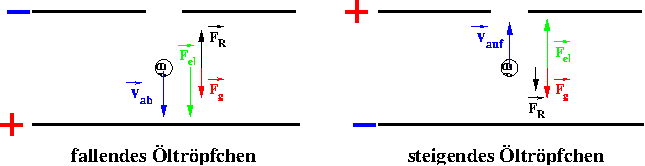
\includegraphics{figures/Abb1.pdf}
    \caption{Kräfte auf ein Öltröpfchen in einem homogenen elektrischen Feld \cite{ap12}.}
    \label{fig:abb1}
\end{figure}


Die elektrostatische Kraft $\vec{F}_\text{el}$ auf ein Teilchen der Ladung $q$ im elektrischen Feld $\vec{E}$ hat die Form 
\begin{equation*}
    \vec{F}_\text{el} = q \vec{E}\, .
    \label{eq:Estat}
\end{equation*}
Ist das Feld parallel zu $\vec{F}_g$, ist die Sinkgeschwindigkeit $\vec{v}_\text{ab}$ größer $v_0$.
Das Kräftegleichgewicht der Sinkmethode hat bei dieser Konfiguration die Form 
\begin{equation}
    \frac{4 \pi}{3} r^3(\rho_\text{Öl} - \rho_\text{L})g - 6 \pi r \eta_\text{L} v_\text{ab} = - q E \, .
    \label{eq:sinkmethode}
\end{equation}
Wenn das elektrische Feld antiparallel zur Gravitationskraft angelegt ist, wirkt es der Gravitationskraft entgegen.
Ist $F_\text{el}$ groß genug, bewegen sich die Öltröpfchen nach oben und es stellt sich ein neues Kräftegleichgewicht mit der Geschwindigkeit $v_\text{auf}$ ein.
Dieses Kräftegleichgewicht der Steigmethode hat die Form
\begin{equation}
    \frac{4 \pi}{3} r^3(\rho_\text{Öl} + \rho_\text{L})g + 6 \pi r \eta_\text{L} v_\text{ab} = + q E \, .
    \label{eq:steigmethode}
\end{equation}

Aus der Sinkmethode \eqref{eq:sinkmethode} und der Steigmethode \eqref{eq:steigmethode} kann die Ladung des beobachteten Öltröpfchen errechnet werden.
Für die Ladung gilt die Gleichung \eqref{eq:ladung}
\begin{equation}
    q = 3 \pi \eta_\text{L} \sqrt{\frac{9}{4} \frac{\eta_\text{L}}{g} \frac{(v_\text{ab} - v_\text{auf})}{(\rho_\text{Öl} - \rho_\text{L})}} \cdot \frac{v_\text{ab}+ v_\text{auf}}{E} ,
    \label{eq:ladung}
\end{equation}
mit dem Tröpfchenradius 
\begin{equation}
    r = \sqrt{\frac{9 \eta (v_\text{ab}-v_\text{auf})}{2 g (\rho_Öl - \rho_\text{L})}}\, .
    \label{eq:rmitEfled}
\end{equation} \\

An dieser Rechnung muss noch eine kleine Korrektur angefügt werden, da die Stokes'sche Reibung nur für Tröpfchen gilt, die größer als die mittlere freie Weglänge in Luft sind.
Diese Voraussetzung ist in diesem Versuch nicht erfüllt. Eine effektive Viskosität wird benötigt
\begin{equation}
    \eta_\text{eff} = \eta_\text{L} \left( \frac{1}{1+ B \frac{1}{p r}}       \right) \, ,
    \label{eq:Veff}
\end{equation}
dabei ist $B = 6,17 \cdot 10^{-3} \text{Torr} \cdot \unit{\centi\meter}$ und p der Luftdruck. Daraus ergibt sich für die korrigierte Ladung
\begin{equation}
    q_{Korr} = q_0 \left(1 + \frac{B}{p r}\right)^{-\frac{3}{2}}  \, ,
    \label{eq:qKorr}
\end{equation}
